\documentclass[9pt,aspectratio=43,mathserif,table]{beamer} 
%  设置为 Beamer 文档类型,设置字体为 10pt,长宽比为16:9,数学字体为 serif 风格
\batchmode
\usepackage{graphicx}
\usepackage{subfigure}
\usepackage{fontspec}
\usepackage{amsmath}

% \setmainfont{Harding Text Web Regular Regular.ttf}
\usepackage{diagbox} % 表头斜线分区
\usepackage{unicode-math}
\usefonttheme{serif}
% \setmathrm{Harding Text Web Regular Regular.ttf} % 设置数学字体为 Times New Roman
\setmathfont{TeX Gyre Termes Math} % 如果您使用 XeLaTeX 或 LuaLaTeX 编译,可以使用其他数学字体
\setmathtt{Courier New} % 设置等宽字体为 Courier New
\setboldmathrm{Times New Roman}
\setmathfont{TeX Gyre Termes Math}[version=bold] % 设置粗体数学字体
\setmathfont{TeX Gyre Termes Math}[range={\mathit}]


\usetheme{Berlin} %主题
\setbeamertemplate{page number in head/foot}[pagenumber]
%\usecolortheme{sustech} %主题颜色

\usepackage[ruled,linesnumbered]{algorithm2e}

\usepackage{fancybox}
\usepackage{xcolor}
\usepackage{listings}

\usepackage{booktabs}
\usepackage{colortbl}

\newcommand{\Console}{Console}
\lstset{ %
	backgroundcolor=\color{white},   % choose the background color
	basicstyle=\footnotesize\rmfamily,     % size of fonts used for the code
	columns=fullflexible,
	breaklines=true,                 % automatic line breaking only at whitespace
	captionpos=b,                    % sets the caption-position to bottom
	tabsize=4,
	commentstyle=\color{mygreen},    % comment style
	escapeinside={\%*}{*)},          % if you want to add LaTeX within your code
	keywordstyle=\color{blue},       % keyword style
	stringstyle=\color{mymauve}\ttfamily,     % string literal style
	numbers=left, 
	%	frame=single,
	rulesepcolor=\color{red!20!green!20!blue!20},
	% identifierstyle=\color{red},
	language=c
}


\definecolor{mygreen}{rgb}{0,0.6,0}
\definecolor{mymauve}{rgb}{0.58,0,0.82}
\definecolor{mygray}{gray}{.9}
\definecolor{mypink}{rgb}{.99,.91,.95}
\definecolor{mycyan}{cmyk}{.3,0,0,0}

%题目,作者,学校,日期
\title{Limit Cycles}
%\subtitle{\fontsize{9pt}{14pt}\textbf{跨临界分岔}}
\author{Speaker: Yichen Lu\quad \newline  \newline \quad }
\institute{\fontsize{8pt}{14pt}}
\date{\today}
\newcommand{\concept}{Limit Cycles}

%学校Logo
%\pgfdeclareimage[height=0.5cm]{sustech-logo}{sustech-logo.pdf}
%\logo{\pgfuseimage{sustech-logo}\hspace*{0.3cm}}

\AtBeginSection[]
{
	\begin{frame}<beamer>
	\frametitle{\textbf{Contents}}
	\tableofcontents[currentsection]
\end{frame}
}
% \beamerdefaultoverlayspecification{<+->}
% -----------------------------------------------------------------------------
\begin{document}
% -----------------------------------------------------------------------------

\frame{\titlepage}

% \section[Contents]{}   %目录
% \begin{frame}{Contents}
% \tableofcontents
% \end{frame}

% -----------------------------------------------------------------------------
\section{Introduction \& Examples}

\begin{frame}
	A \textbf{limit cycle} is an isolated closed trajectory.

	\begin{figure}[H]
		\centering
		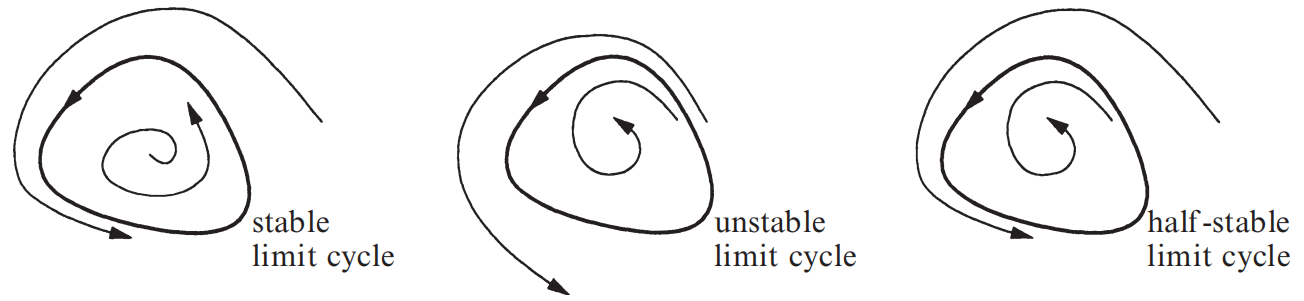
\includegraphics[width=\textwidth]{fig701.jpg}
	\end{figure}

	\begin{figure}
		\centering
		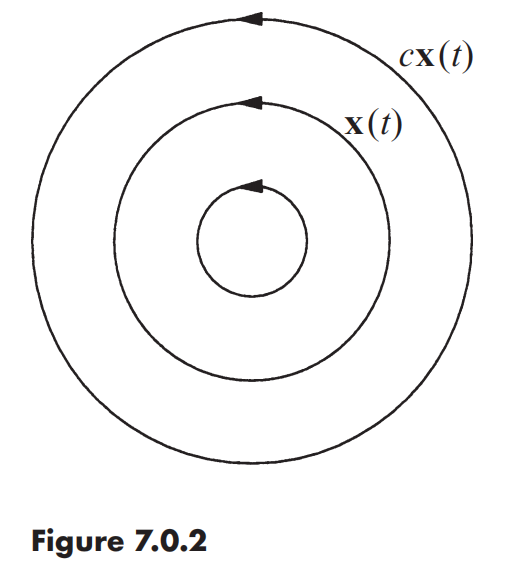
\includegraphics[width=0.3\textwidth]{fig702.jpg}
	\end{figure}
\end{frame}


\begin{frame}
	Consider the system
	$$
	\dot{r}=r\left( 1-r^2 \right) ,  \dot{\theta}=1  \left( r\ge 0 \right) 
	$$
	\begin{figure}
		\centering
		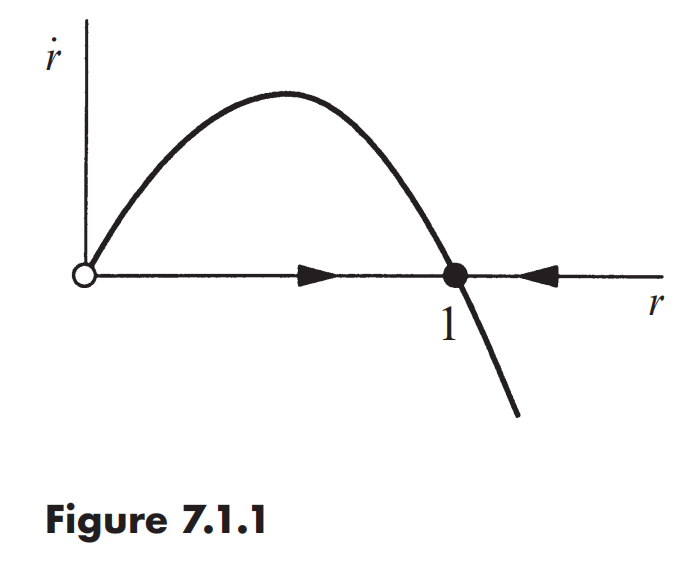
\includegraphics[width=0.45\textwidth]{fig711.jpg}
	\end{figure}

\end{frame}


\begin{frame}
	\begin{figure}
		\centering
		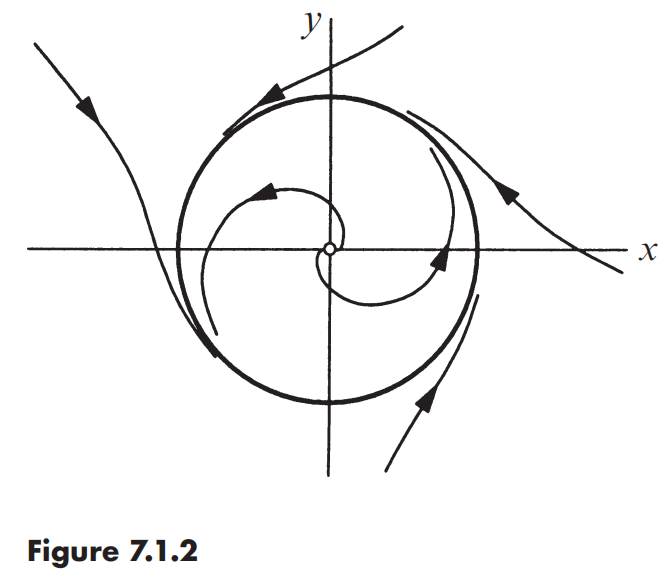
\includegraphics[width=0.35\textwidth]{fig712.jpg}
	\end{figure}

	we plot $x(t) = r(t)\cos\theta (t)$
	
	\begin{figure}
		\centering
		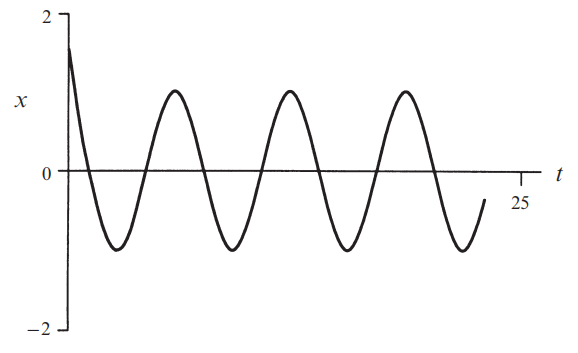
\includegraphics[width=0.35\textwidth]{fig713.jpg}
	\end{figure}

	so $x(t)=\cos(t + \theta_0)$ is a solution of the system.
\end{frame}

\begin{frame}{van der Pol equation}
	$$
	\ddot{x}+\mu \left( x^2-1 \right) \dot{x}+x=0
	$$
	$\mu \left( x^2-1 \right)$ is a \textbf{nonlinear damping}, This term acts like ordinary positive damping for $|x|< 1$, but like negative damping for $|x| > 1$.

	\begin{figure}
		\centering
		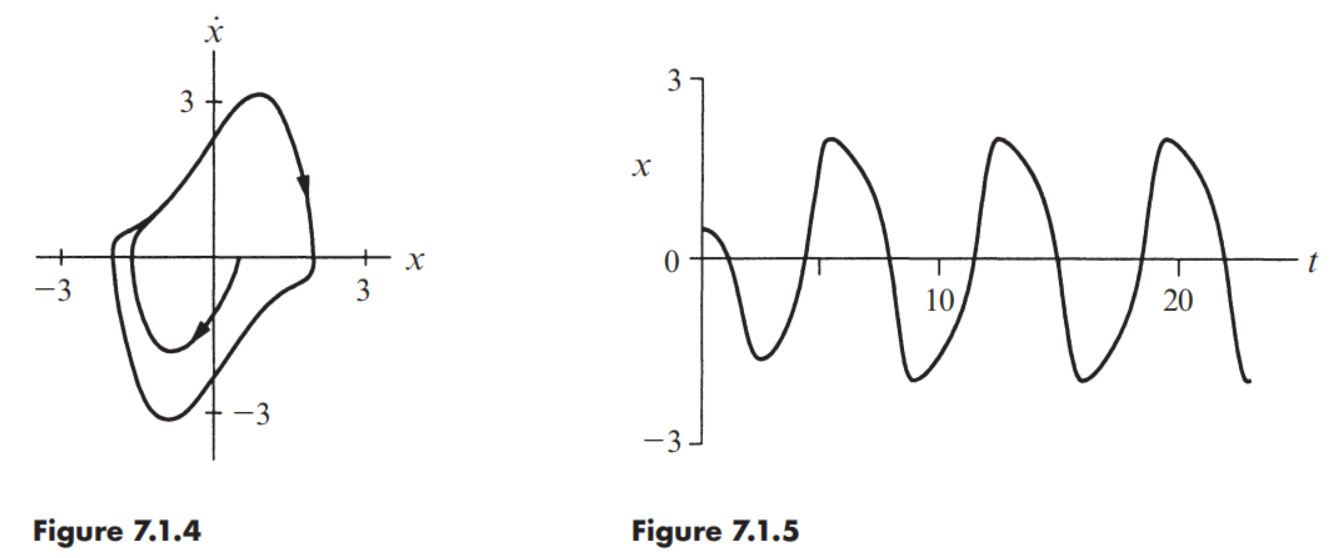
\includegraphics[width=0.85\textwidth]{fig714.jpg}
	\end{figure}

\end{frame}

\section{Ruling Out Closed Orbits}
\begin{frame}{Gradient Systems}
	A \textbf{gradient system} with \textbf{potential function} $V$, if the system can be written in $\dot{x}=-\nabla V(x)$.

	$ $

	\textbf{Theorem 7.2.1: } Closed orbits are impossible in gradient systems.

	$ $

	\textbf{Proof:}
	$$
	\begin{aligned}
		\Delta V&=\int_0^T{\frac{dV}{dt}\mathrm{dt}}\\
		&=\int_0^T{\left( \nabla V\cdot \dot{x} \right) dt}\\
		&=-\int_0^T{\left\| \dot{x} \right\| ^2dt}\\
		&<0\\
	\end{aligned}
	$$


\end{frame}

\begin{frame}
	\textbf{Example 7.2.1}
	$$
	\begin{aligned}
		\dot{x}&=\sin y\\
		\dot{y}&=x\cos y\\
	\end{aligned}
	$$

	We can find a potential function $V(x, y) = -x \sin y$, satisfy $\dot{x}=-\partial V/\partial x$ and $\dot{y}=-\partial V/\partial y$, so the system is a gradient system.

	$ $

	\textbf{Example 7.2.2}
	The nonlinearly damped oscillator $\ddot{x} + (\dot{x})^3 + x=0$ has no periodic solutions.
	$$
	E(x, \dot{x})=\cfrac{1}{2}(x^2+\dot{x}^2)
	$$
	$$
	\dot{E}=\dot{x}(x+\ddot{x})=\dot{x}(-\dot{x}^3)=-\dot{x}^4\le0
	$$
	$$
	\Delta E=\int_0^T{\dot{E}dt}=-\int_0^T{\dot{x}^4dt}\le0
	$$
\end{frame}


\section{glossary}
\begin{frame}{glossary}
	\begin{itemize}
			\item \textbf{Limit cycle} is an isolated closed trajectory.
			\item \textbf{Nonlinear damping item} This term acts like ordinary positive damping for some situations, but like negative damping for other situations.
			\item \textbf{Gradient system} is a system that can be written in $\dot{x}=-\nabla V(x)$.
	\end{itemize}
\end{frame}
% -----------------------------------------------------------------------------
\end{document}
